% The MIT License (MIT)
% =====================

% **Copyright (c) 2018 Anish Athalye (me@anishathalye.com)**

% Permission is hereby granted, free of charge, to any person obtaining a copy of
% this software and associated documentation files (the "Software"), to deal in
% the Software without restriction, including without limitation the rights to
% use, copy, modify, merge, publish, distribute, sublicense, and/or sell copies
% of the Software, and to permit persons to whom the Software is furnished to do
% so, subject to the following conditions:

% The above copyright notice and this permission notice shall be included in all
% copies or substantial portions of the Software.

% THE SOFTWARE IS PROVIDED "AS IS", WITHOUT WARRANTY OF ANY KIND, EXPRESS OR
% IMPLIED, INCLUDING BUT NOT LIMITED TO THE WARRANTIES OF MERCHANTABILITY,
% FITNESS FOR A PARTICULAR PURPOSE AND NONINFRINGEMENT. IN NO EVENT SHALL THE
% AUTHORS OR COPYRIGHT HOLDERS BE LIABLE FOR ANY CLAIM, DAMAGES OR OTHER
% LIABILITY, WHETHER IN AN ACTION OF CONTRACT, TORT OR OTHERWISE, ARISING FROM,
% OUT OF OR IN CONNECTION WITH THE SOFTWARE OR THE USE OR OTHER DEALINGS IN THE
% SOFTWARE.


% Gemini theme
% https://github.com/anishathalye/gemini

\documentclass[final]{beamer}

% ====================
% Packages
% ====================

\usepackage[T1]{fontenc}
\usepackage{lmodern}
\usepackage[size=custom,width=130 ,height=95,scale=1.0]{beamerposter}
\usetheme{gemini}
\usecolortheme{gemini}
\usepackage{graphicx}
\usepackage{booktabs}
\usepackage{tikz}
\usepackage{pgfplots}
\usepackage{tcolorbox}
\usepackage{geometry}

% ====================
% Lengths
% ====================

% If you have N columns, choose \sepwidth and \colwidth such that
% (N+1)*\sepwidth + N*\colwidth = \paperwidth
\newlength{\sepwidth}
\newlength{\colwidth}
\setlength{\sepwidth}{0.025\paperwidth}
\setlength{\colwidth}{0.3\paperwidth}

\newcommand{\separatorcolumn}{\begin{column}{\sepwidth}\end{column}}

% ====================
% Title
% ====================

\title{Enabling Reproducible Microbiome Science through \\ Decentralized Provenance Tracking in QIIME 2}

\author{Christopher R. Keefe \and Ahmad Turan Naimey \and J. Gregory Caporaso (advisor)}

\institute[shortinst]{The Pathogen and Microbiome Institute at Northern Arizona University}

% ====================
% Body
% ====================

\begin{document}

\begin{frame}[t]
\begin{columns}[t]
\separatorcolumn

\begin{column}{\colwidth}

  \begin{block}{Objective and Introduction}

    \textbf{Objective:} To demonstrate the ways in which automatic, integrated, decentralized
    provenance tracking in QIIME 2 \cite{framework|qiime2:2018.8.0.dev0+1.g2788661|0} enables reproducible microbiome science,
    using a sample analysis as framework for discussion.

    \textbf{QIIME 2 Key Features:}
    \begin{itemize}
      \item Integrated and automatic tracking of data provenance
      \item Semantic type system
      \item Plugin system for extending microbiome analysis functionality
      \item Support for multiple types of user interfaces (e.g. API, command line, graphical)
    \end{itemize}
  \end{block}

  \begin{block}{Creating a QIIME 2 artifact = initiating provenance tracking}

   In order to work in QIIME 2, we must first import our data to create a new
   QIIME 2 artifact. We then demultiplex our data, passing the new artifact
   into \code{q2-demux}, alongside a column of sample metadata containing
   barcode sequences.

   \begin{tcolorbox}
   [width=\textwidth, colframe=blue]
   {A QIIME 2 \code{Artifact} is an immutable collection of data and its associated
           metadata, including the \textit{type}, \textit{format}, and \textit{provenance} (Figure \ref{fig:provenance}).
   Using Artifacts rather than plain files helps QIIME 2 ensure actions
   performed are meaningful. Each action generates new artifacts whose
   provenance metadata includes a comprehensive history of the data in the
   artifact, including:}
    \begin{itemize}
      \item {the processes to which the data was subjected}
      \item {all parameters chosen when running these processes}
      \item {citation information relevant to the methods chosen}
      \item {version information for all software involved (QIIME 2 and all relevant plugins)}
    \end{itemize}
    \end{tcolorbox}
  \end{block}

  \begin{block}{QIIME 2 analyses are host-agnostic}

    De-noising the data will be computationally intensive, so we use a
    high-performance cluster. (Figure \ref{fig:dada2})

    \begin{figure}[tph!]
      {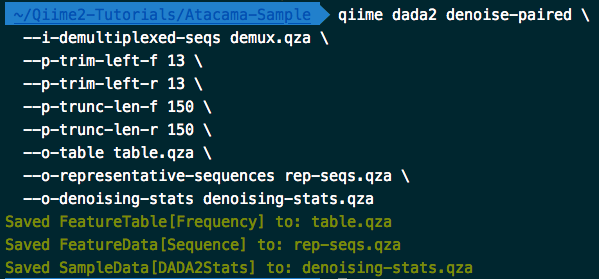
\includegraphics[width=18cm, height=8cm]{assets/dada2}}
      \caption{DADA2 denoising in q2cli}
      \label{fig:dada2}
    \end{figure}

    \begin{tcolorbox}
    [width=\textwidth, colframe=blue]
    {The integrated and decentralized handling of provenance metadata in
    artifacts makes it easy for QIIME 2 users to transfer files and run jobs
    through any QIIME 2 interface on any host, accumulating and retaining
    accurate accurate provenance information}.
  \end{tcolorbox}

  \end{block}

  \begin{block}{QIIME 2 analyses are interface-agnostic}
    Automatic provenance tracking saves time and alleviates uncertainty.

    \begin{enumerate}
      \item Investigate alpha and beta diversity using the Artifact API in
      a Jupyter Notebook \cite{PER-GRA:2007} (Figure \ref{fig:taxabar})
      \item Subsequent analysis is handled in QIIME 2 Studio, a GUI
      that provides asynchronous process handling and access to all
      QIIME 2 plugins in our environment (Figure \ref{fig:q2studio})
    \end{enumerate}

    \begin{tcolorbox}
    [width=\textwidth, colframe=blue]
    {Throughout this complex analysis, QIIME 2 records our methods.
    The provenance data in our artifacts and visualizations minimizes
    uncertainty about which file is correct}.
    \end{tcolorbox}

    \begin{figure}[tph!]
      {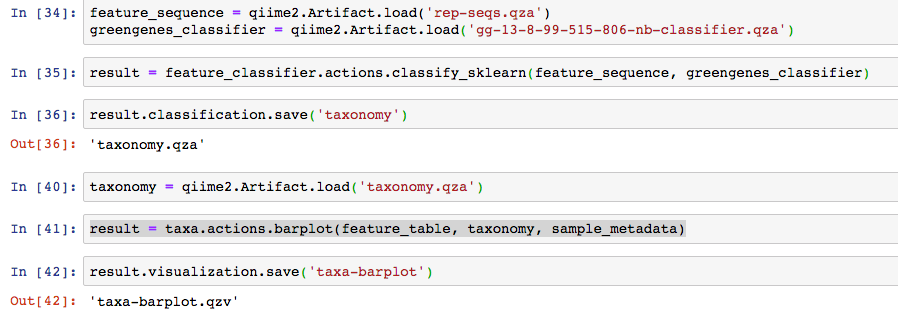
\includegraphics[width=25cm]{assets/taxabar}}
      \caption{Jupyter Notebook}
      \label{fig:taxabar}
    \end{figure}

  \end{block}

\end{column}

\separatorcolumn

\begin{column}{\colwidth}

  \begin{block}{Visualizations}
    \begin{figure}[tph!]
      {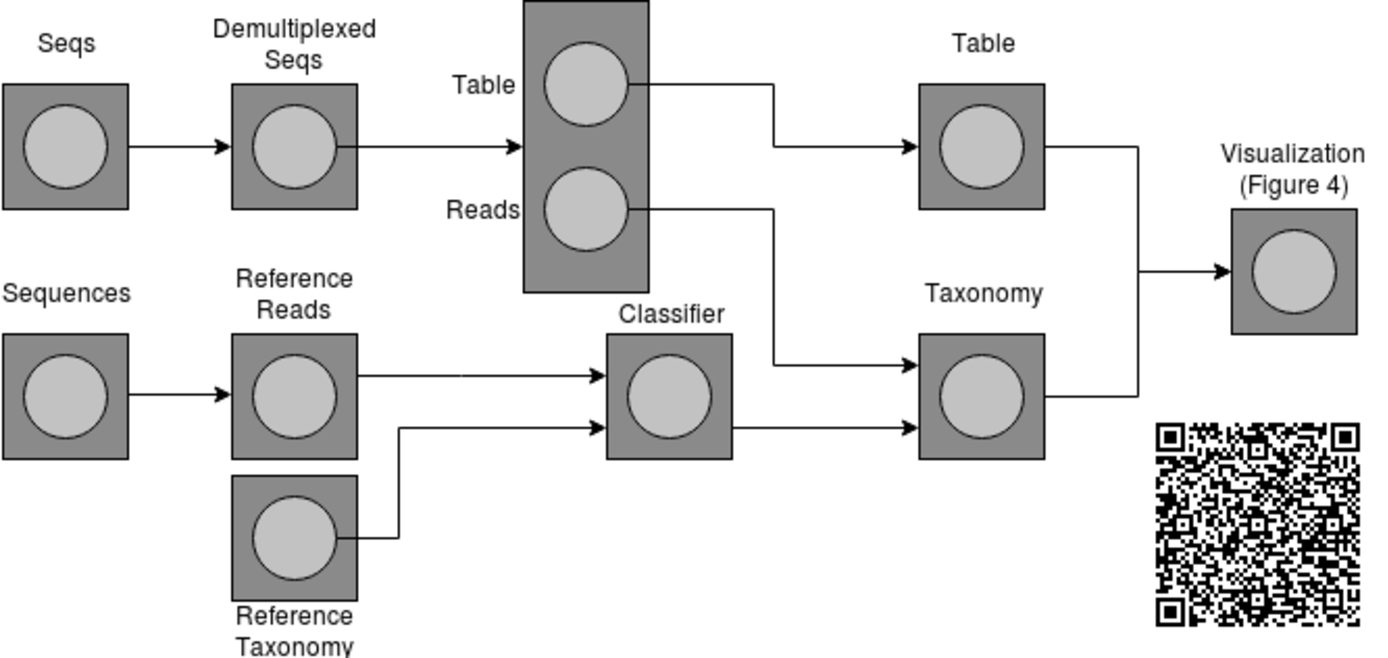
\includegraphics[width=\linewidth]{assets/provenance}}
      \caption{Provenance tree in QIIME 2}
      \label{fig:provenance}
    \end{figure}

    \begin{figure}[tph!]
      {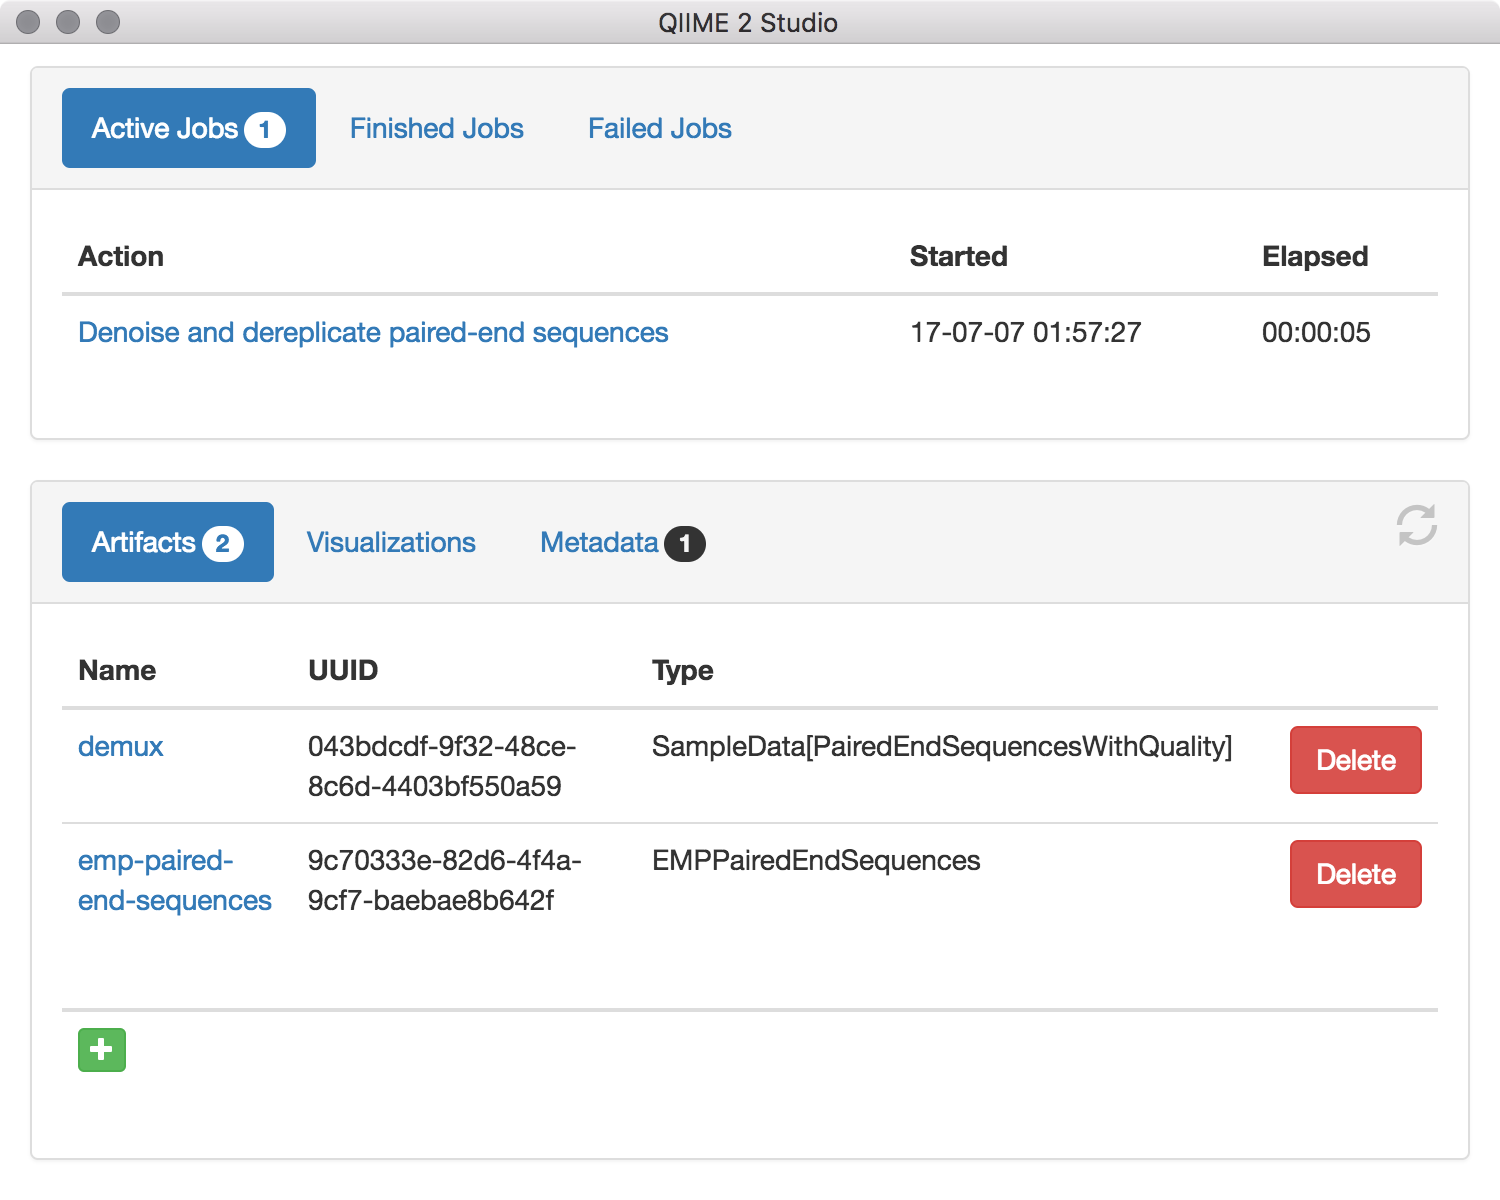
\includegraphics[height=18cm]{assets/q2studio}}
      \caption{QIIME 2 Studio}
      \label{fig:q2studio}
    \end{figure}

    \begin{figure}[tph!]
      {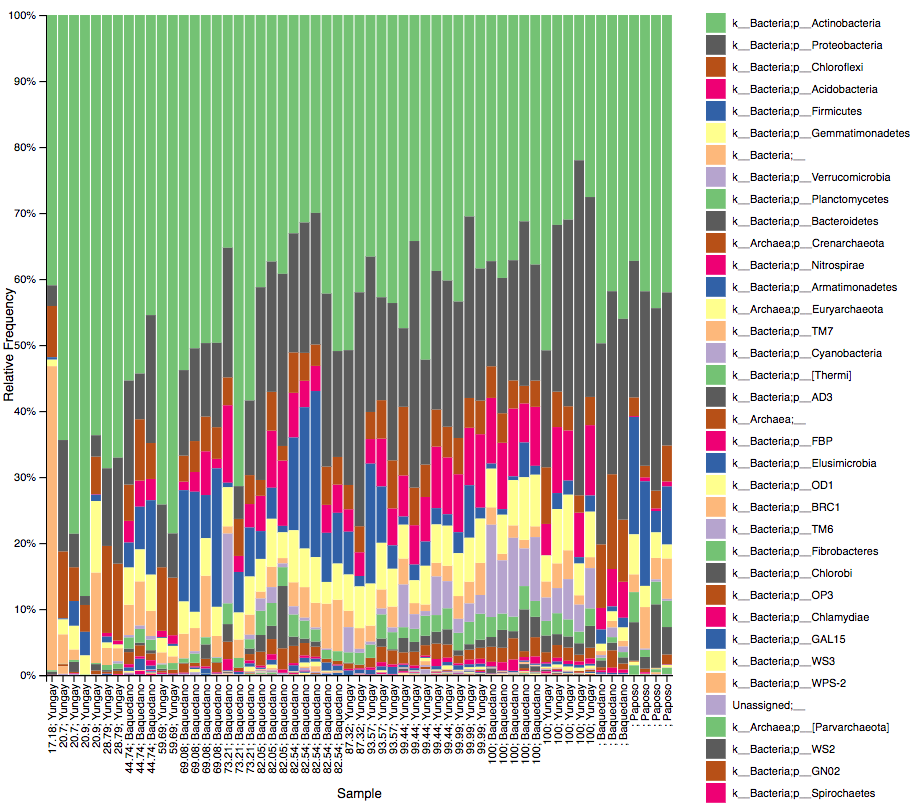
\includegraphics[width=\linewidth]{assets/taxabar-plot}}
      \caption{Taxa-bar Plot}
      \label{fig:taxabar-plot}
    \end{figure}
  \end{block}

  \begin{block}{Our Analysis and the Atacama Study}
    The analysis which frames this poster is based on work by Neilson et al in
    “Significant Impacts of Increasing Aridity on the Arid Soil Microbiome”
    \cite{Neilsone00195-16}. This study documents correlations between aridity
    and changes in the soil microbiome along two arid-to-hyperarid transects in
    the Atacama Desert, Chile. For new users interested in understanding
    our approach, a tutorial based on this study is available in the
    QIIME 2 docs.
  \end{block}

\end{column}

\separatorcolumn

\begin{column}{\colwidth}

    \begin{block}{Sharing QIIME 2 visualizations}
      QIIME 2 visualizations can be shared and viewed without a software
      install, and contain complete provenance information.

    \begin{enumerate}
      \item Interactive visualizations play a significant role in understanding and
      communicating our data. (Figure \ref{fig:taxabar-plot})
      \item QIIME 2’s provenance graphs allow us to review which methods and
      parameters were used, simplifying creation of an accurate methods section
      and supplementary materials.
      \item We generate the citations for this poster with \code{qiime tools citations}
      \item We submit, confident that our reported methods are accurate, our
      visualizations represent our final experimental methods, and our
      citations are appropriate and complete.
      \item Reviewers use https://view.qiime2.org to confirm methods and outcomes are
      aligned, without the need to download any special software. (Figure 6)
    \end{enumerate}

    \begin{tcolorbox}
    [width=\textwidth, colframe=blue]
    {By packaging data with provenance, QIIME 2 reduces the risk that the
    methods used to produce a given outcome are accidentally misreported.
    QIIME 2 has integrated citation information into plugins, allowing
    researchers to export citations as BibTeX}.
    \end{tcolorbox}


    \begin{figure}[tph!]
      {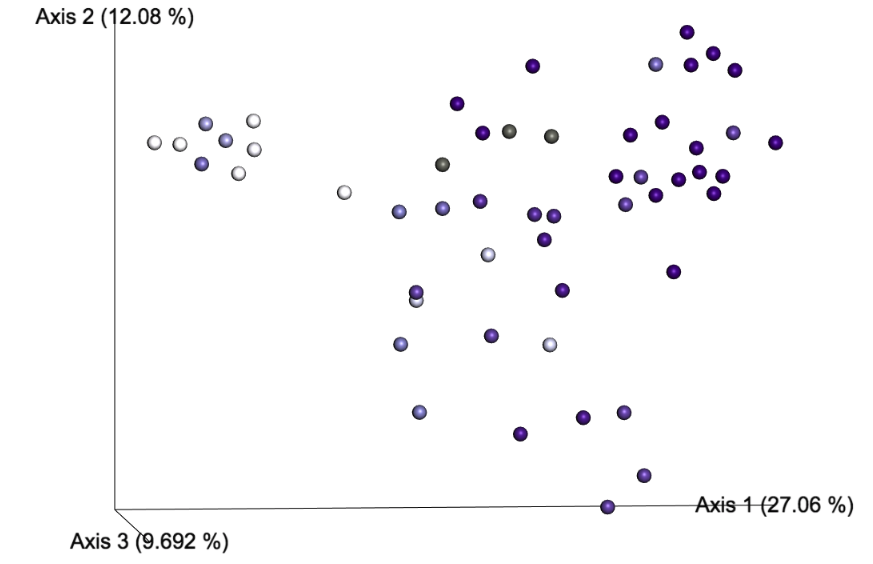
\includegraphics[height=17cm]{assets/emperor}}
      \caption{Emperor visualization in q2view}
      \label{fig:emperor}
    \end{figure}

  \end{block}

  \begin{block}{Decentralized provenance tracking enables study \\ reproduction, replication \& extension}

    QIIME 2’s provenance metadata makes it easy for anyone to reproduce our
    computational analysis independently to confirm the quality of our results.
    Should we choose to expand our study, or conduct further research using
    similar methods, provenance graphs provide a “road map”.

  \end{block}

  \begin{block}{Future Work}

    \begin{itemize}
      \item \textbf{Allow QIIME 2 to consume provenance metadata:} Reading
      provenance \textit{into} QIIME 2 could allow for computer-assisted
      introspection into research methods, automated transcription of methods
      for publication, and auto-generation of “pipeline” scripts for common workflows.
      \item \textbf{QIIME 2 Studio and HPC:} In the future, we hope that QIIME 2 Studio might interact
      directly with HPC schedulers, to simplify the process of connecting with
      and running computationally-intensive processes remotely.
    \end{itemize}

  \end{block}

  \begin{block}{References}

    \nocite{*}
    \bibliographystyle{acm}\bibliography{poster}

  \end{block}

\end{column}

\separatorcolumn
\end{columns}
\end{frame}

\end{document}
